
\documentclass[10pt,a4paper]{article}
\usepackage[utf8]{inputenc}
\usepackage[french]{babel}
\usepackage[left=2cm,right=2cm,top=2cm,bottom=2cm]{geometry}
\usepackage{hyperref}
\usepackage{graphicx}

%opening
\title{TP 2}
\author{Nicolas Vadkerti}
\usepackage{listings} % Required for inserting code snippets
\usepackage[usenames,dvipsnames]{color} % Required for specifying custom colors and referring to colors by name

\definecolor{DarkGreen}{rgb}{0.0,0.4,0.0} % Comment color
\definecolor{highlight}{RGB}{255,251,204} % Code highlight color

\lstdefinestyle{Style1}{ % Define a style for your code snippet, multiple definitions can be made if, for example, you wish to insert multiple code snippets using different programming languages into one document
language=Perl, % Detects keywords, comments, strings, functions, etc for the language specified
backgroundcolor=\color{highlight}, % Set the background color for the snippet - useful for highlighting
basicstyle=\footnotesize\ttfamily, % The default font size and style of the code
breakatwhitespace=false, % If true, only allows line breaks at white space
breaklines=true, % Automatic line breaking (prevents code from protruding outside the box)
captionpos=b, % Sets the caption position: b for bottom; t for top
commentstyle=\usefont{T1}{pcr}{m}{sl}\color{DarkGreen}, % Style of comments within the code - dark green courier font
deletekeywords={}, % If you want to delete any keywords from the current language separate them by commas
%escapeinside={\%}, % This allows you to escape to LaTeX using the character in the bracket
firstnumber=1, % Line numbers begin at line 1
frame=single, % Frame around the code box, value can be: none, leftline, topline, bottomline, lines, single, shadowbox
frameround=tttt, % Rounds the corners of the frame for the top left, top right, bottom left and bottom right positions
keywordstyle=\color{Blue}\bf, % Functions are bold and blue
morekeywords={}, % Add any functions no included by default here separated by commas
numbers=left, % Location of line numbers, can take the values of: none, left, right
numbersep=10pt, % Distance of line numbers from the code box
numberstyle=\tiny\color{Gray}, % Style used for line numbers
rulecolor=\color{black}, % Frame border color
showstringspaces=false, % Don't put marks in string spaces
showtabs=false, % Display tabs in the code as lines
stepnumber=5, % The step distance between line numbers, i.e. how often will lines be numbered
stringstyle=\color{Purple}, % Strings are purple
tabsize=2
}

\newcommand{\insertcode}[2]{\begin{itemize}\item[]\lstinputlisting[caption=#2,label=#1,style=Style1]{#1}\end{itemize}} 


% \insertcode{"Scripts/example.pl"}{Nena would be proud.} 

\begin{document}

\maketitle


\url{https://github.com/SlaynPool/CR_SEOC2/}
\section{Données météorologiques locales}

Dans  cette  première  étape,  nous  nous  intéresserons à  l’acquisition  des  données  météorologiques actuelles. Nous souhaitons obtenir la température et l’humidité relative (degré d’hygrométrie). Pour cela, nous utiliserons le composant DHT11 fourni dans votre kist.
\subsection{Effectuer  une  recherche  rapide  sur  le  fonctionnement  de  ce  composant  et  indiquer  clairement comment peut-on le relier à notre carte de développement (faire un schéma).}
Nous trouvons la datasheet du composant ici: \url{https://www.mouser.com/datasheet/2/758/DHT11-Technical-Data-Sheet-Translated-Version-1143054.pdf}
A la page 5, nous y trouvons ceci, ce qui nous indique comment cabler le composant à notre ESP32.
\begin{figure}[h!]
\centering
 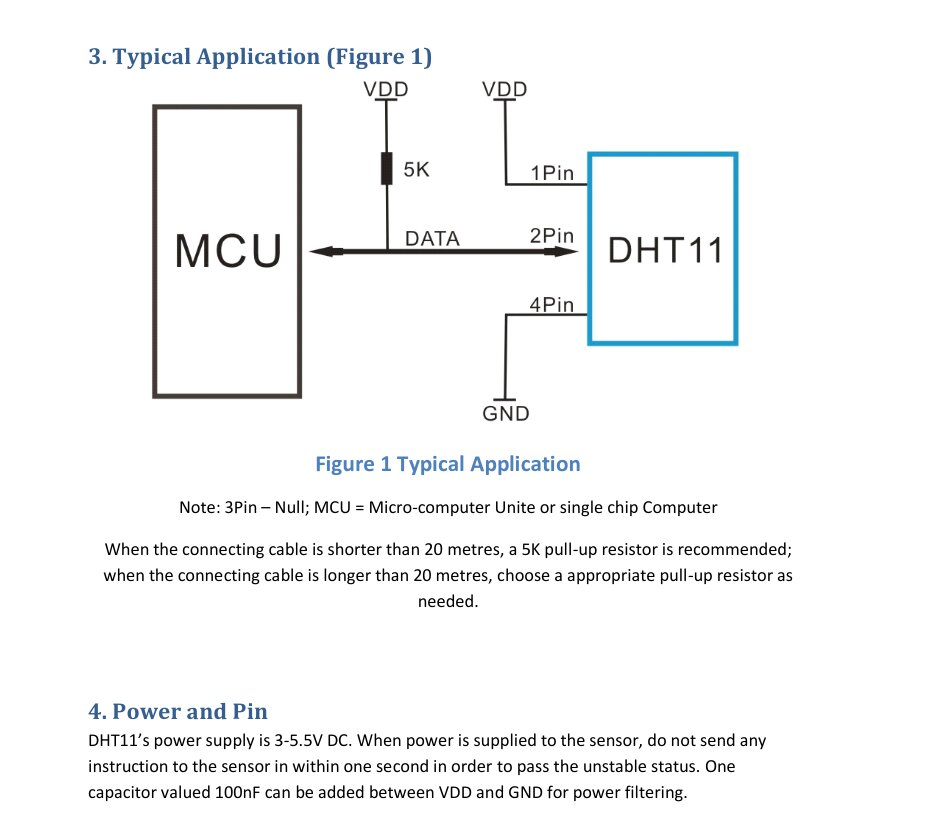
\includegraphics[scale=0.3]{image/1.jpg}
\caption{Documentation }
\label{fig:net }
\end{figure}\\
En pratique, voici ce que cela donne sur une bredboard:
\begin{figure}[h!]
\centering
 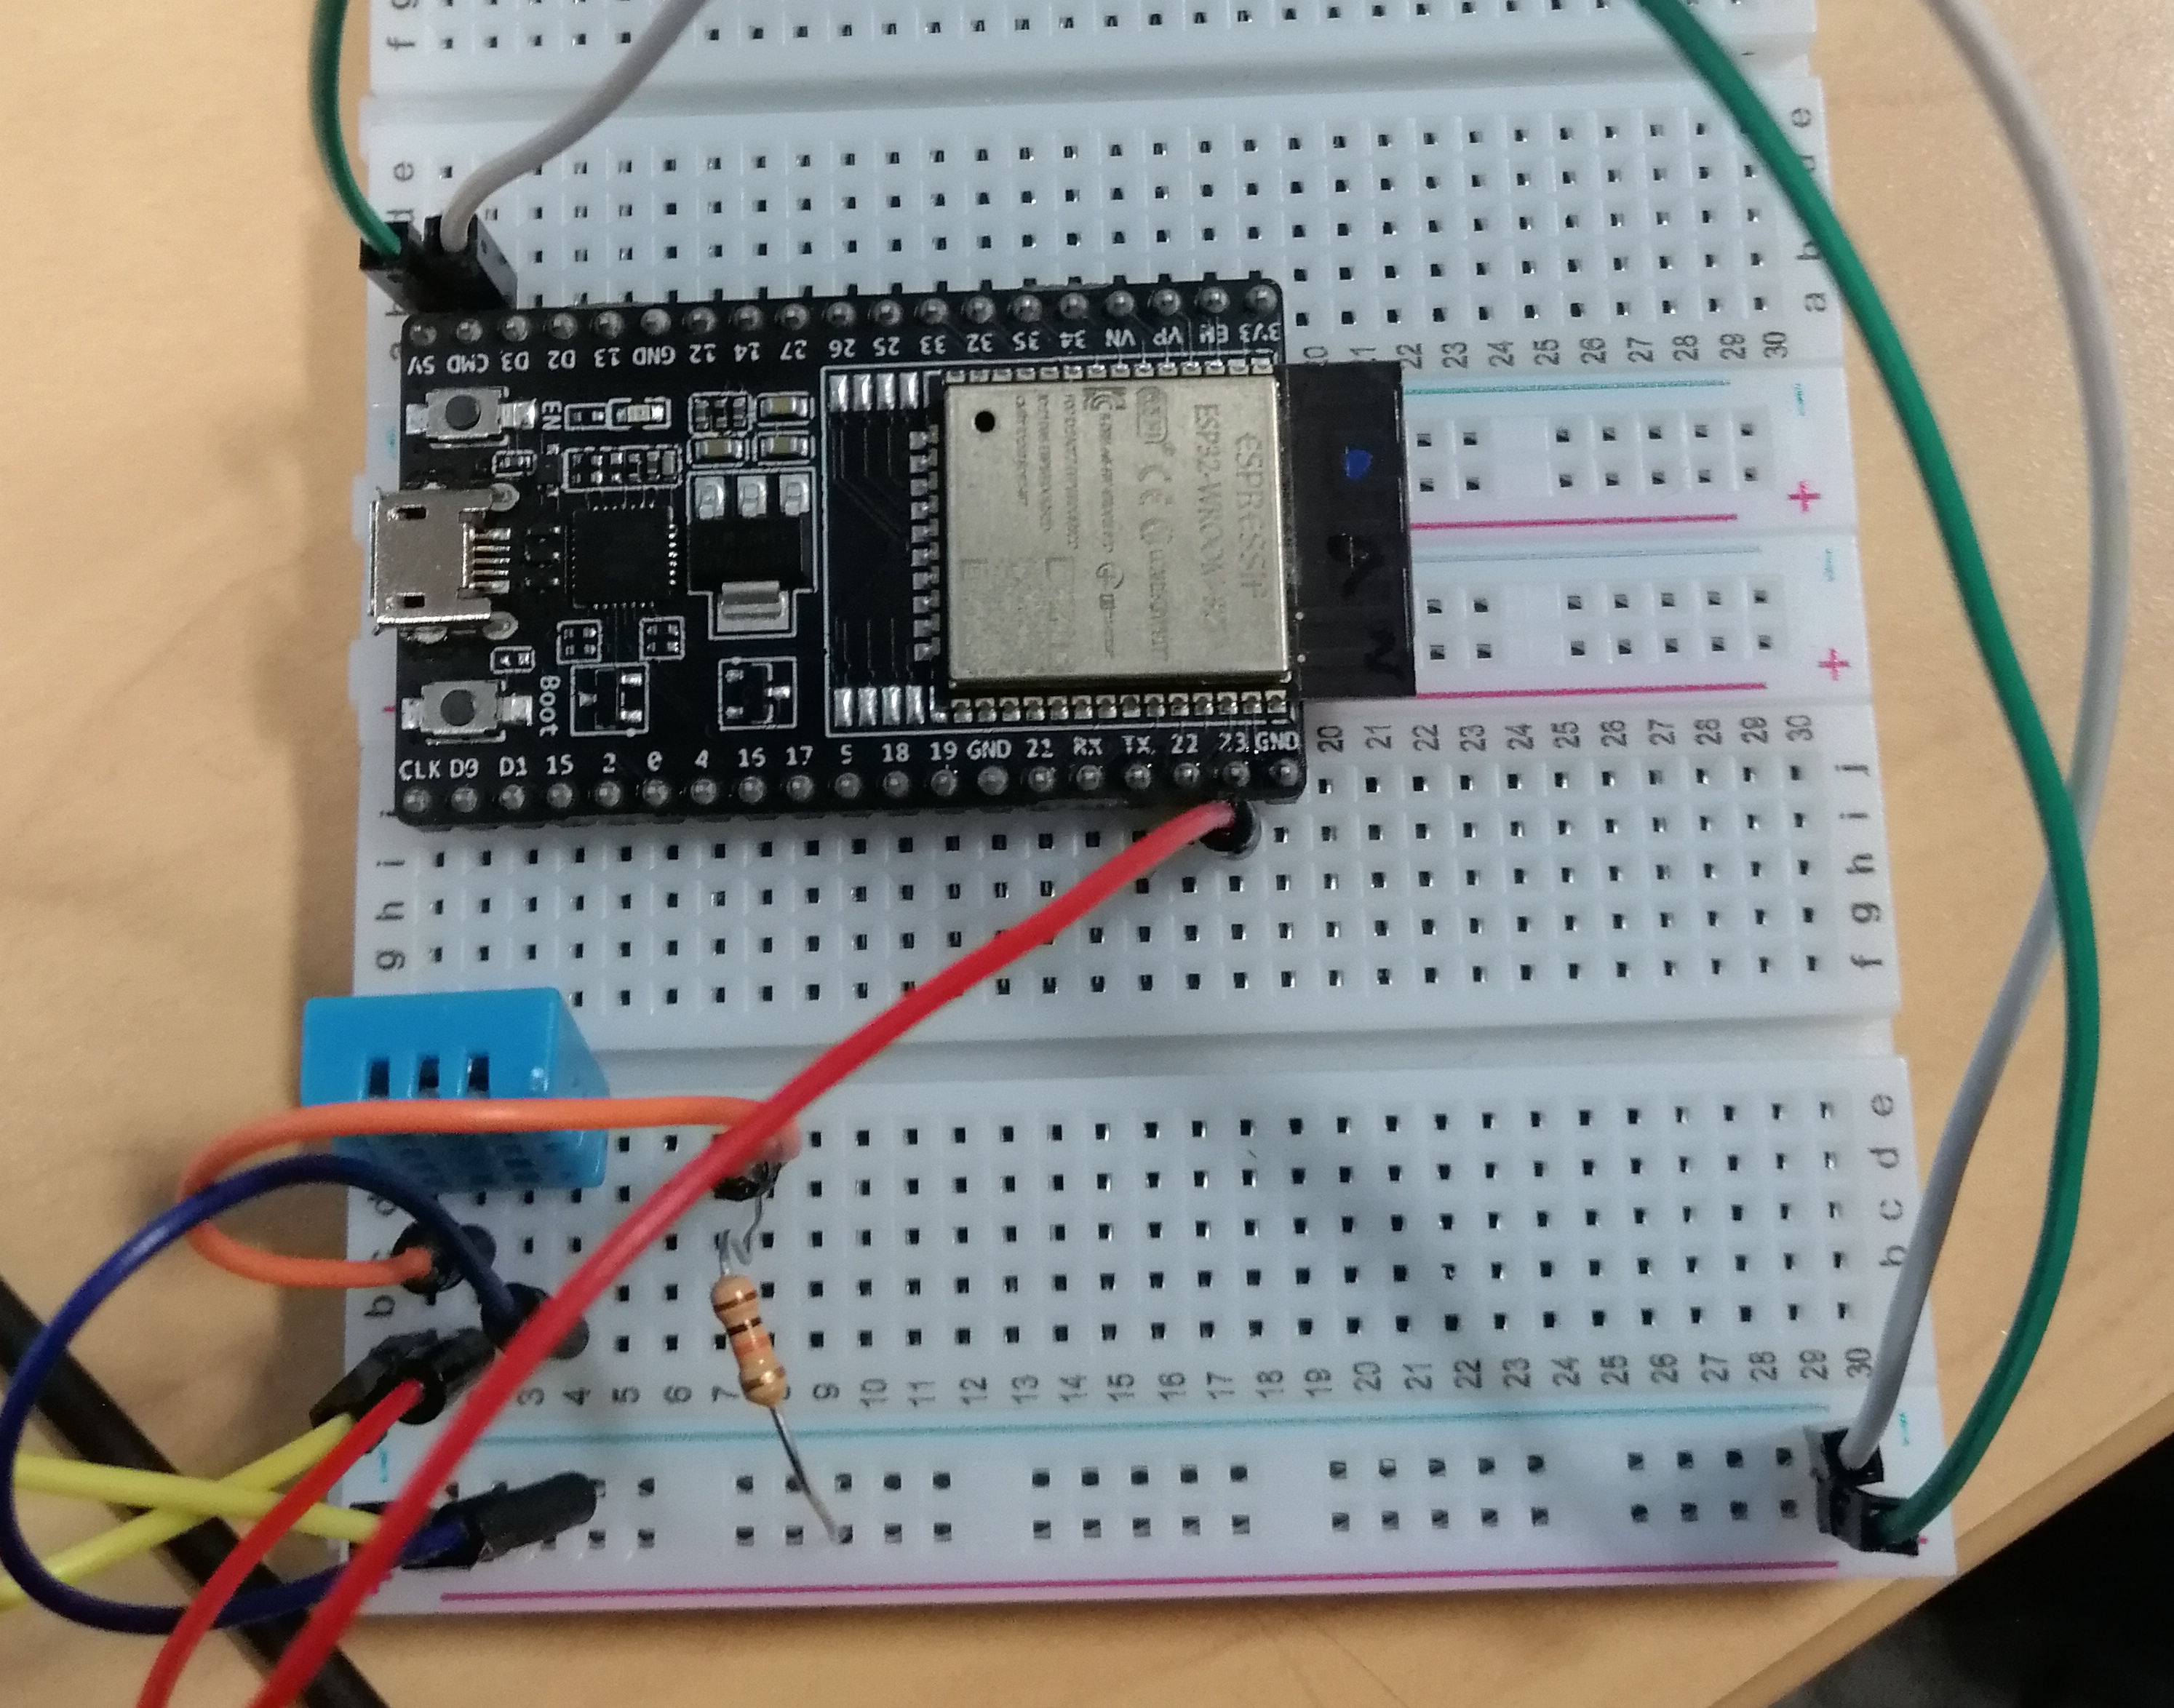
\includegraphics[scale=0.15]{image/2.jpg}
\caption{Pratique}
\label{fig:net }
\end{figure}\newpage
 \subsection{Télécharger  la  librairie  nécessaire  au  bon  fonctionnement  du  DHT11  et  écrire  un  programme permettant  d’afficher  sur  une  console  de  votre  ordinateur,  toutes  les  5  secondes,  la  température actuelle et le degré d’hygrométrie.}
 La librairie que nous allons utiliser est celle -ci: \url{https://github.com/adafruit/DHT-sensor-library}\\
 Puis nous allons utiliser le sketch d'exemple fournis pour tester notre montage:
 \insertcode{code/dht11/dht11.ino}{Le sketch exemple}
 Voici un extrait du port serie :
 \insertcode{code/1.txt}{STDOUT}
Le dispositif fonctionne correctement, en effet lorsque je souffle de l'air chaud dessus, les valeurs augmentes significativement.

\section{Prévision météorologiques }
 L'api de OpenWeather permet de récupérer des informations sur les  prévisions  météorologiques.
 L'idée de fonctionnement de l'API est de faire une requette http à la bonne URL, et nous recevrons un fichier JSON qui contiendra les informations qui nous intérèssent.
 Par exemple, grâce à cette URL:\url{https://api.openweathermap.org/data/2.5/weather?id=2992165&appid=MaCleAPI}
 Nous recevrons les informations météos de la ville de Montpellier
Pour les prévisions de Montpellier:
\url{https://api.openweathermap.org/data/2.5/forecast?id=2992165&appid=MaCleAPI}

Pour faire ceci sur l'ESP32, Nous allons avoir besoins: 
\begin{itemize}
 \item une connection wifi/Accées à internet.
\item Un Parser JSON. Lien utile: \url{https://arduinojson.org/v6/assistant/}
\end{itemize}
\insertcode{code/forecast.ino}{Prévision }
Résultat:
\insertcode{code/2.txt}{resultat}

\subsection{ Compléter le programme par l’affichage d’une comparaison entre la température et l’hygrométrie actuelles mesurées localement et celles obtenues vie l’API.}
Pour cela, nous allons récuperer l'ID de la ville de béziers : 6455063
Nous voulons les données actuelles donc notre requete sera :
\url{https://api.openweathermap.org/data/2.5/weather?id=6455063&appid=MaCleAPI}
Et donc voici le code pour l'ESP32:
\insertcode{code/comparaison.ino}{Comparaison}

On inclue l'ecran LCD :

\begin{figure}[h!]
\centering
 \includegraphics[scale=0.1]{image/3.jpg}
\caption{Pratique}
\label{fig:net }
\end{figure}\newpage
Ainsi que le code qui va avec :
\insertcode{code/LCD.ino}{LCD}
\begin{figure}[h!]
\centering
 \includegraphics[scale=0.1]{image/4.jpg}
\caption{Pratique}
\label{fig:net }
\end{figure}\newpage
\end{document}

